%%%%%%%%%%%%%%%%%%%%%%%%%%%%%%%%%%%%%%%%%%%%%%%%%%%%%%%%%%%%%%%%%%% 
%                       rpithes-short.tex                         %
%         Template for a short thesis all in one file             %
%        (titlepage info below assumes masters degree}            %
%  Just run latex (or pdflatex) on this file to see how it looks  %
%      Be sure to run twice to get correct TOC and citations      %
%%%%%%%%%%%%%%%%%%%%%%%%%%%%%%%%%%%%%%%%%%%%%%%%%%%%%%%%%%%%%%%%%%% 
%
%  To produce the abstract title page followed by the abstract,
%  see the template file, "abstitle-mas.tex"
%
%%%%%%%%%%%%%%%%%%%%%%%%%%%%%%%%%%%%%%%%%%%%%%%%%%%%%%%%%%%%%%%%%%%

\documentclass{thesis}
\usepackage{graphicx}   % if you want to include graphics files

% Use the first command below if you want captions over 1 line indented.
% A side effect of this is to remove the use of bold for captions. 
% To restore bold, also include the second line below.
%\usepackage[hang]{caption}     % to indent subsequent lines of captions
%\renewcommand{\captionfont}{\bfseries} % only needed with caption package;
                                        %   otherwise bold is default)
                                        
%%%%%%%%%%%%%%%%%%%%  supply titlepage info  %%%%%%%%%%%%%%%%%%%%%
\thesistitle{\bf NSL Spindle\\Map-Reduce at the Edge In a V2V Environment}        
\author{William Rory Kronmiller}        
\degree{Master of Science}
\department{Computer Science} % provide your area of study here; e.g.,
%  "Mechanical Engineering", "Nuclear Engineering", "Physics", etc.
\thadviser{Dr. Stacy Patterson}
%\cothadviser{First co-adviser} %if needed
%\cocothadviser{Second co-adviser} % if needed
%  For a masters project use \projadviser instead of \thadviser, 
%  and \coprojadviser and \cocoprojadviser if needed. 
\submitdate{March 3\\(For Graduation May 2017)}        
%\copyrightyear{1685}  % if date omitted, current year is used. 
%%%%%%%%%%%%%%%%%%%%%   end titlepage info  %%%%%%%%%%%%%%%%%%%%%%
      
\begin{document} 
\titlepage             % Print titlepage   
%\copyrightpage        % optional         
\tableofcontents       % required 
\listoftables          % required if there are tables
\listoffigures         % required if there are figures

\specialhead{ACKNOWLEDGMENT}
The acknowledgment text goes here. Unlike chapter headings, 
this heading is not numbered.
% Personal thing

\specialhead{ABSTRACT}
Write your abstract here. Again, the heading does receive a number.

\chapter{INTRODUCTION}
%TODO(MEETING): explain WHY we care about sparse vs. dense, why we care about different window sizes
    % amount of batching
    %NOTE: this could go in introduction paragraph
%TODO
The text of the first chapter goes here. To cite a reference for the
bibliography, use a command such as:\cite{thisbook}
\section{A Section Heading}
This is a sentence to take up space and look like text.
\subsection{A Subsection Heading}

\chapter{Background and Related Work}
%TODO
%TODO: need to explain how spark works, how akka works, 

%TODO: related works (mention that C-DRIVE came up with clustered architecture)

%

\chapter{System Architecture}
    Spindle provides a novel streaming data processing platform by building on
    existing cutting edge and industry standard distributed systems, primarily
    from the Apache ecosystem. 

    The Spindle system consists of three major components: a set of Apache Spark %TODO: cite
    streaming programs managed by one or more clients, a custom data ingestion and
    query management Middleware, and edge computing software running on network
    connected vehicles.
    
    Spindle operates on the vehicle level as a Scala
    \cite{scala} program running on the Akka \cite{akka} framework; this program
    is responsible for handling cluster formation, data collection, and edge
    computation.

    Data passes through components of the Vehicle software in the form of 
    messages sent to Kafka \cite{kafka} topics. Similarly, data is transferred
    at the cloud layer using Kafka.

    Clients receive data from the middleware as Kafka messages that a custom Spark \cite{spark}
    library processes into DStream tuples which can be further processed using any of the available
    Spark streaming operations written for DStreams and RDDs.

\section{Theorized Architecture}
    %TODO: walk through spark query, middleware update, propagation through vehicle networks, vehicle-level-map, clusterhead-reduce, transmission to middleware, transmission to spark streaming, secondary reduce, etc..

%TODO
% DO THIS NEXT
% Ask braden what good vis tools are out there

% Want sequence diagram for a single map-reduce step
% Component diagrams showing communications
% Focus more on envisioned 
% Follow Cloud Computing papers for format (upper bound on page count is 5-10 pages)

%separate sections for envisioned architecture and for test design ("accommodations for testing")

\chapter{Experiments}
\section{Data Sets}
\subsection{Vehicle Traces}
   The Spindle experiments depend on a set of vehicle traces 
   generated using "the open source vehicular network simulation framework" VEINS, which simulates
   vehicle movement and radio connectivity in a "realistic" manner \cite{veins}. The VEINS traces
   were generated by Mike Wittie of the Montana State University as part of a larger overall research
   project. 
   The traces come in the form of sharded CSV files containing time-series mappings of three different types:
   speed, x-position, y-position, and connectivity to other vehicles. Each time-series mapping includes
   a timestamp, a vehicle uid, and a value (speed, position, reachable-vehicle-id). 
   These shards have been parsed into a Postgres database with a table for each mapping type.
   %TODO(MEETING): insert information about City of Cologne 
   % insert information about node count, length of time here
   % Saw we pick sparse, dense region, etc... here (move from subsection below)
\subsection{Test Regions} %TODO(MEETING): make sub-sub section of Vehicle traces subsection
    \paragraph{Original VEINS Traces}
    %TODO (MEETING): insert VEINS visualization here
        The original VEINS traces span a region from $(41735, 85178.4)$ to $(63071.5, 114426)$ and includes 3340 distinct
        vehicles. This dataset includes more vehicles than the current simulator implementation can handle due to the large
        number of threads, network connections, and Kakfa topics that would be required (the thread/topic count scales with the
        number of vehicles multiplied by a constant multiple of the average number of map/reduce queries running on each node).
        A real-world deployment would distribute the threads/topics over the set of vehicles in the system such that each
        vehicle and kafka cluster would have threads and topics proportional to the number of active map/reduce queries.
        In essence, this is a temporary limitation of the simulation architecture, not the real-world architecture.

        To overcome the simulator's limitations, we defined two test regions, one dense region and one sparse region
        being transited by approximately the same number of vehicles. The sparse and dense regions were selected based
        on the number of vehicles transiting them and based on the layout of the underlying road networks.

    \begin{figure}
        \centering
        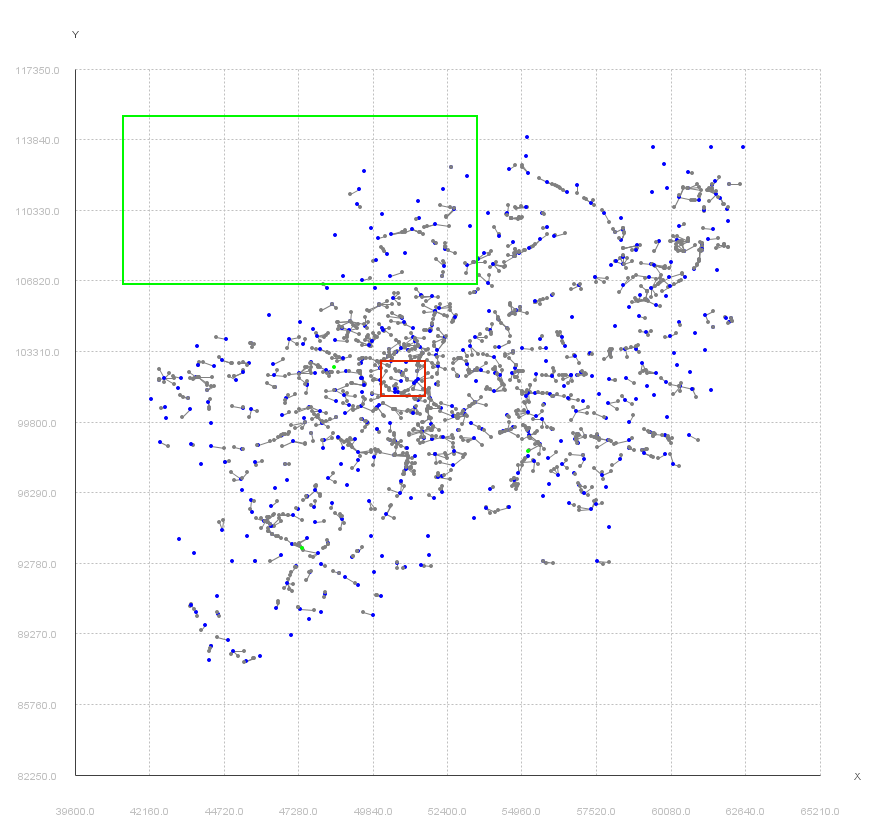
\includegraphics[scale=.5]{sparse-and-dense-clusters.png}
        \caption{Illustration of VEINS Vehicles with MANET Clustering, Courtesy Xiaotian Duan}
        \label{fig:regions}
    \end{figure}
    \paragraph{Sparse Region}
        The sparse region is transited by 148 distinct vehicles over the course of the simulation and defines a bounding
        box from $(40000, 106800)$ to $(53000, 114000)$. The sparse region covers an area on the outskirts of the city,
        with a relatively low density of vehicles. The sparse region is illustrated by a green box in \ref{fig:regions}.
    \paragraph{Dense Region}
        The dense region defines a bounding box from $(50000, 100000)$ to $(51000, 102000)$ and is transitied by
        131 vehicles over the course of the simulation. The dense region covers a small area near the city center
        where the density of vehicles is higher. The dense region is illustrated by a red box in \ref{fig:regions}.

\subsection{Window Sizes}
    Kafka Streams can perform reduce operations over messages received over the course of a user-defined time-window
    and will write the results to a KTable, a logical structure whose API approximates that of a key-value store. %TODO: citations
    Spindle's Kafka Streams reducer adds a \verb|Batcher|, which transmits the final value of a time-window's KTable
    entry to some destination Kafka topic (in this case the middleware). As such, Spindle supports micro-batch operations
    on Kafka streams with user-configurable window sizes. The sizes tested were 10, 15, and 30 seconds.
\subsection{Test Clusters}
    The cluster head assignments for each node are pre-computed using either Xiaotian's %TODO: cite Xiaotian
    clustering algorithm or some base-line \verb|single_clusterhead| (all vehicles in simulation share a single clusterhead)
    or \verb|self_clusters| (all vehicles act as their own cluster heads).
\subsection{Clustering Algorithms}
    The spindle architecture takes advantage of work done by fellow RPI student Xiaotian Duan on generating
    clusters of vehicles based on vehicle connectivity and lane position. 
    %TODO: get permission from Xiaotian for using clustering images
    %TODO: include information about cluster density for each clustering (sparse/dense)
    %TODO: Fix the quotes!

\section{Test Software}
    \paragraph{SpindleSim}
        The Spindle simulator (SpindleSim) is implemented in several thousand lines of Scala %TODO: cite
        and is implemented on top of the Akka %TODO: cite
        actor model framework. The Scala/Akka portions of the simulator implement as realistically
        as is practical the software that would run on a real-world deployment of Spindle. This is
        accomplished by creating a separate Akka actor for each simulated vehicle, where each actor
        is given a cache of time-series simulation events and data and a connection to a ``World''
        actor responsible for keeping track of global simulation time; this global time-keeper 
        can be thought of as a stand-in for a GPS clock running on each vehicle. Each vehicle
        actor is then responsible for managing its publish-subscribe streams and messages, as well
        as its simulated connections to other vehicles in its cluster. Messages are exchanged between
        vehicles and send from vehicles to ``the cloud" by way of special "Stream Relay" Kakfa Streams
        programs responsible for filtering expired and "Canary" messages %TODO: explain redundant messages in architecture
        and responsible for keeping a running sum of the number of bytes sent on a per-relay basis and logging
        these sums to separate CSV files at run-time.
    \paragraph{AutoSim}
        The Scala/Akka simulator (SpindleSim) currently has a number of pre-configured map/reduce jobs written
        that can be turned on or off using the program's \verb|application.conf| file. A secondary
        program, dubbed AutoSim, runs the simulator iteratively, writing to the conf file, launching
        SpindleSim, then gathering the results and uploading them to a database and permanent storage.
        In order to iterate through the desired test configurations, AutoSim reads from a table \verb|sim_configs_vx| in a 
        Postgres 9.6.1 database hosted on an AWS EC2 \verb|m4.large| reserved instance.
        AutoSim will choose among the least-tested configurations in the configs table, write the configuration to
        the SpindleSim \verb|application.conf|, and launch an instance of SpindleSim. While SpindleSim is running, AutoSim
        greps the console logs for exception messages. If an exception is detected, the current SpindleSim instance is killed
        and a notification is sent via AWS SNS topic reporting the error message in order to facilitate debugging. If the SpindleSim
        operation completes, AutoSim uploads the CSV logs to an AWS S3 bucket and parses the final message byte sums from the CSV
        files then writes the results to a \verb|sim_results_vx| table in Postgres. AutoSim is a simple Node.JS ES6 application
        that is run from the Babel-Node %TODO: CITE
        transpiler.
    \paragraph{Environment}
        AutoSim and SpindleSim are packaged inside a docker image, \\\verb|wkronmiller/nsl-spindle-simulator| that can be run from
        a laptop, desktop, or EC2 instance. The test framework and container are designed to survive the total loss of local
        storage and/or the running simulator container by storing the results of all completed simiulation operations on
        S3 and a remote database. This design decision allows the test framework to be run on an AWS EC2 Spot Fleet %TODO: citation
        which offers discounts of roughly 70-90\% in exchange for the requirement that any software running on a Spot instance
        be designed to killed at any time with little or no warning. %TODO citation
        The architecture also enables trivial transfer of the simulator across different machines, easing debugging and mitigating
        problems related to transient EC2 network problems. 
\section{Test Configurations}
\subsection{Example Map/Reduce Programs}
    \paragraph{speedSum}
        The most simple map/reduce operation tested is the "speedSum" job, which simply maps each vehicle's available data to a
        tuple containing only the vehicle's speed. The reduce operation run at the clusterheads takes the sum of the speeds
        of each of the cluster member vehicles.
%TODO (MEETING): each paragraph should be formatted as: use case, query format
        % first sentence - query computes x
        % follow-on: uses this map function, uses reduce function
    \paragraph{geoFiltered}
        This map/reduce job extends speedSum by performing a word-count-style map operation that maps each vehicle's sensors
        to the vehicle count and the vehicle speed: \verb|(1, [speed])|. The reduce operation again simply sums the count
        and speed of each member vehicle \verb|([numVehiclesInCluster], [sumOfSpeeds])|. The geoFiltered query also is selective,
        in that for a given test region the geoFiltered query operates only on a subset of the test region containing approximately
        half of the vehicles being tested.
    \paragraph{geoMapped}
        The geoMapped query performs a similar map/reduce operation to geoFiltered, but instead of filtering out half the
        test region, the geoMapped query maps half the test region to one region ID and maps the other half of the
        test region to a second region ID, then performs a reducebykey. The map operation produces the following:
        \verb|(regionId) -> (1, [speed])| and the reduce produces \verb|(regionId) -> ([numVehiclesInCluster], [sumOfSpeeds])|.

\section{Simulator Results}
    %TODO
    %GRAPHING:
        % Generating six figures
        % Message sizes:
            % Normalize with 1 being message sizes with single clusterhead
            % Plotting percentage savings with separate bars for dense/sparse wehre dense/sparse are normalized separately
        % Total bandwidth:
            % Total for dense with and without clustering
            % Total for sparse with and without clustering
        % Can include stddev bars
        % Annotate graphs with things like "this shows a reduction..."
            % try to give intuition as to why
    % maybe look at variance in data sent at clusterhead 
%TODO

\chapter{Conclusion}
%TODO: what did we do/show?
\section{Future Work}
%TODO

%\chapter{THE NEXT CHAPTER}
%And so on, for more chapters.
%Another citation for the bibliography:\cite{anotherbook}

% The following produces a numbered bibliography where the numbers
% correspond to the \cite commands in the text.
\specialhead{LITERATURE CITED}
\begin{singlespace}
\begin{thebibliography}{99}
\bibitem{thisbook} This is the first item in the Bibliography.
Let's make it very long so it takes more than one line.
Let's make it very long so it takes more than one line.
\bibitem{anotherbook} The second item in the Bibliography.
%%% TEMPLATE END
\bibitem{veins}
    http://veins.car2x.org %TODO: proper citation format (Feb 22, 17)
\bibitem{scala}
    http://www.scala-lang.org %TODO: proper citation format Feb 26, 17
\bibitem{akka}
    http://akka.io % Feb 26
\bibitem{kafka}
    https://kafka.apache.org % Feb 26
\bibitem{spark}
    http://spark.apache.org/streaming/ %Feb 26
\end{thebibliography}
\end{singlespace}

%%%%%%%%%%%%%%%%%%%%%%%  For Appendices  %%%%%%%%%%%%%%%%%%%
\appendix    % This command is used only once!
\addtocontents{toc}{\parindent0pt\vskip12pt APPENDICES} %toc entry, no page #
\chapter{THIS IS AN APPENDIX}
Note the numbering of the chapter heading is changed.
This is a sentence to take up space and look like text.
\section{A Section Heading}
This is how equations are numbered in an appendix:
\begin{equation}
x^2 + y^2 = z^2
\end{equation} 

\chapter{THIS IS ANOTHER APPENDIX}
This is a sentence to take up space and look like text.

\end{document}
